\documentclass[ma3408.tex]{subfiles}
\begin{document}
\chapter{Spectral sequences}
Spectral sequences are a powerful computation tool in topology. Computing with spectral sequences is a bit like computing integral in calculus; it is helpful to have ingenuity and a big bag of tricks - and even that may not be enough! 
\section{Filtered complexes}
We begin our discussion on spectral sequences by discussing filtered complexes. 
\begin{Rem}
Let $C_{\bullet}$ be a chain complex and $F_0C_{\bullet}$ a sub-complex. Then we have a short exact sequence 
\[
0 \to F_0C_{\bullet} \to C_{\bullet} \to C_{\bullet}/F_0C_{\bullet} \to 0
\]
which gives rise to a long exact sequence in homology 
\[
\cdots \to H_i(F_0C_{\bullet}) \to H_i(C_{\bullet}) \to H_i(C_{\bullet}/F_0C_{\bullet}) \xrightarrow{\partial} H_{i-1}(F_0C_{\bullet}) \to \cdots
\]
Suppose we know $H_*(F_0C_{\bullet})$ and $H_*(C_{\bullet}/F_0C_{\bullet})$. Can we compute $H_*(C_{\bullet})$? We can split the long exact sequence into short exact sequences 
\[
0 \to \coker(\partial) \to H_*(C_{\bullet}) \to \ker(\partial) \to 0 
\]
which gives the following procedure for computing $H_*(C_{\bullet})$:
\begin{enumerate}
	\item Compute $H_*(F_0C_{\bullet})$ and $H_*(C_{\bullet}/F_0C_{\bullet})$
	\item Consider the two-term chain complex
\[
H_*(C_{\bullet}/F_0C_{\bullet}) \xrightarrow{\partial} H_*(F_0C_{\bullet}).
\]
Denote its homology groups by $G_1H_*$ and $G_0H_*$. 
\item
There is a short exact sequence
\[
0 \to G_0H_* \to H_*(C_{\bullet}) \to G_1H_* \to 0. 
\]
This determines $H_*(C_{\bullet})$ up to extension.\sidenote{This is a common phenomenon for a spectral sequence. For example, if we have a short exact sequence $0 \to \bbZ/2 \to M \to \bbZ/2 \to 0$, can you say what the middle group is? Not without further information!}
\end{enumerate}
How would we handle the situation if we have a longer filtration: $\cdots F_pC_{\bullet} \subseteq F_{p+1}C_{\bullet} \subseteq \cdots$?

\begin{Exa}
Consider a (semi-simplicial) model of the $2$-sphere $S^2$ with vertices $\{a,b,c\}$, edges $\{A,B,C\}$ and solid triangles $\{P,Q\}$ and with inclusions as soon in \Cref{fig:s2}.\sidenote{This example comes from Example 2.1 of \url{https://arxiv.org/pdf/1702.00666.pdf}.}
\begin{figure}[h!] \centering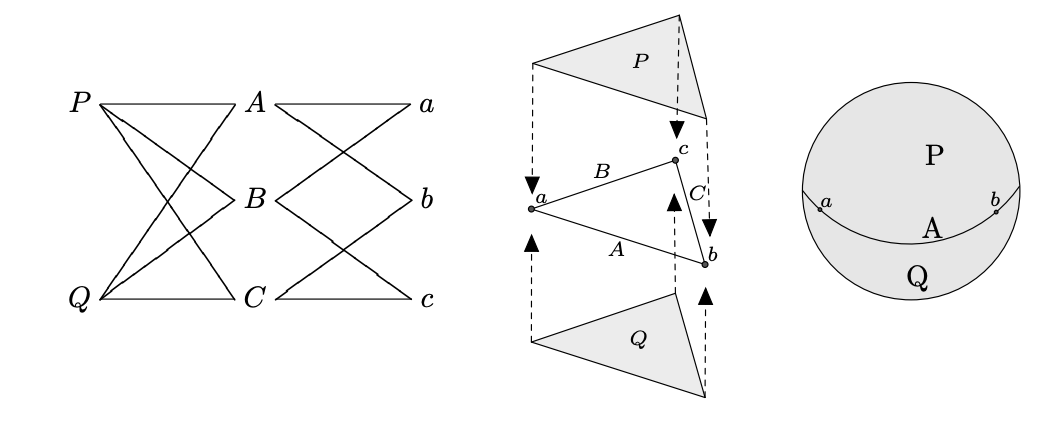
\includegraphics[scale = 0.5]{s2.png}\caption{Simplicial model of $S^2$}\label{fig:s2}\end{figure}
The associated chain complex is $C_{\bullet}$
\[
0 \to \bbZ\{ P, Q\} \xrightarrow{d} \mathbb{Z}\{A,B,C\} \xrightarrow{d} \bbZ\{a,b,c\} \to 0
\]
with
\[
d(P) = C-B+A \quad d(Q) = C-B+A
\]
and
\[
d(A) = b-a \quad d(B) = c-a \quad d(C) = c-b.
\]
One can check directly that $H_i(C_{\bullet};\bbZ) \cong \bbZ$ for $i = 0,2$ and is zero otherwise. Alternatively, we use the following filtration:
\[
\xymatrix@C=10pt@R=0pt{
0\ar[r] &\bbZ\{P,Q\}\ar[r]& \bbZ\{A,B,C\}\ar[r] & \bbZ\{a,b,c\}\ar[r]& 0\\
0\ar[r] &0\ar[r]& \bbZ\{A,B\}\ar[r] & \bbZ\{a,b,c\}\ar[r]& 0\\
0\ar[r] &0\ar[r]& \bbZ\{A\}\ar[r] & \bbZ\{a,b\}\ar[r]& 0.\\
}
\]
The differentials are induced from $d_1$ and $d_2$ and a direct check shows that they are still chain complexes. Passing to the quotient, we get a chain complex we call $E_0$:
\[
\xymatrix@C=10pt@R=0pt{
0\ar[r] &\bbZ\{P,Q\}\ar[r]& \bbZ\{C\}\ar[r] & 0\ar[r]& 0&&d_0(P)=C,d_0(Q)=C\\
0\ar[r] &0\ar[r]& \bbZ\{B\}\ar[r] & \bbZ\{c\}\ar[r]& 0&&d_0(B)=c\\
0\ar[r] &0\ar[r]& \bbZ\{A\}\ar[r] & \bbZ\{a,b\}\ar[r]& 0&&d_0(A)=b-a.\\
}
\]
Taking homology with respect to $d_0$ we obtain $E^1$:
\[
\xymatrix@C=10pt@R=0pt{
0\ar[r] &\bbZ\{P-Q\}\ar[r]& 0 \ar[r] & 0\ar[r]& 0\\
0\ar[r] &0\ar[r]& 0\ar[r] & 0\ar[r]& 0\\
0\ar[r] &0\ar[r]& 0\ar[r] & \bbZ\{\bar a\}\ar[r]& 0.\\
}
\]
The general theory of spectral sequences will tell us that we have computed the homology of $H_*(C_{\bullet})$; there is a $\bbZ$ in degree 2, generated by $P-Q$ and a $\bbZ$ in degree 0, generated by $\bar a$. 
\end{Exa}
\end{Rem}
This leads us to the theory of filtered modules. 
\begin{Def}
	A filtered $R$-module is an $R$-module $A$ together with an increasing sequence of submodules $F_pA \subseteq F_{p+1}A$ indexed by $p \in \mathbb{Z}$ such that $\cup_{p} F_pA = A$ and $\cap_{p} F_pA = \{ 0 \}$. The filtration is bounded if $F_pA = \{ 0 \}$ for $p$ sufficiently small, and $F_pA = A$ for $p$ sufficiently large. The associated graded module is defined by 
	\[
G_pA = F_pA/F_{p-1}A.
	\]
\end{Def}
\begin{Def}
	A filtered chain complex is a chain complex $(C_{\bullet},\partial)$ together with a filtration $\{ F_pC_i \}$ of each $C_i$ such that the differential preserves the filtration: $\partial(F_pC_i) \subseteq F_p C_{i-1}$. Then, $\partial$ induces $\partial \colon G_p C_i \to G_pC_{i-1}$ on the associated graded modules. 
\end{Def}
\begin{Rem}
	The filtration on $C_{\bullet}$ induces a filtration on the homology of $C_{\bullet}$ by
	\[
F_pH_i(C_{\bullet}) = \{ \alpha \in H_i(C_{\bullet}) \mid \exists x \in F_pC_i, \alpha = [x] \}.
	\]
	This has associated graded pieces $G_pH_i(C_{\bullet})$. 
\end{Rem}
\begin{Rem}
Suppose we want to compute $H_*(C_{\bullet})$ and that we can compute the homology of the associated graded pieces $H_*(G_pC_{\bullet})$. Does this determine $G_pH_*(C_{\bullet})$? This leads to the idea of the spectral sequence of a filtered complex. 
\end{Rem}
\section{The spectral sequence of a filtered complex}
\begin{Def}
Let $(F_pC_{\bullet},\partial)$ be a filtered chain complex. Let us write
\[
E^0_{p,q} \coloneqq G_pC_{p+q} = F_pC_{p+q}/F_{p-1}C_{p+q}.
\]
The differential $\partial$ induces a differential on $E^0$,
\[
\partial_0 \colon E^0_{p,q} \to E^0_{p,q-1}.
\]
We denote the homology of the associated graded by
\[
E^1_{p,q} \coloneqq H_{p+q}(G_pC_{\bullet},\partial_0).
\]
\end{Def}
\begin{Rem}
We can think of $E^1_{p,q}$ as a "first order approximation" to $H_*(C_{\bullet})$. We can also define a differential
\[
\partial_1 \colon E^1_{p,q} \to E^1_{p-1,q}
\]
as follows: a homology class $\alpha \in E^1_{p,q}$ can be represented by a chain $x \in F_pC_{p+1}$ such that $\partial x \in F_{p-1}C_{p+q-1}$. We define $\partial_1(\alpha) = [\partial x]$. Because $\partial^2 = 0$, we can check that $\partial_1^2 = 0$ and that $\partial_1$ is well defined. 
\end{Rem}
\begin{Def}
With notation as above, we define
\[
E_2^{p,q} = \ker(\partial_1 \colon E^1_{p,q} \to E^1_{p-1,q})/\im(\partial_1 \colon E^1_{p+1,q} \to E^1_{p,q}). 
\]
\end{Def}
\begin{Rem}
We can continue this procedure, and define an "r"-th order approximation to $G_pH_{p+q}(C_{\bullet})$ by
\[
E^r_{p,q} = \frac{x \in F_pC_{p+q} \mid \partial x \in F_{p-r}C_{p+q-1}}{F_{p-1}C_{p+q} + \partial(F_{p+r-1}C_{p+q+1}}).
\]
The notation denotes the quotient of the numerator by the intersection with the denominator. 

So instead of considering cycles, we consider chains in $F_p$ whose differentials vanishes "to order r", and instead of modding out by the entire image, we only mod out by $\partial(F_{p+r-1})$. 
\end{Rem}
The main result regarding these groups is the following. 
\begin{Lem}\label{lem:ss_filtered_complex}
Let $(F_pC_{\bullet},\partial)$ denote a filtered chain complex, and define $E^r_{p,q}$ as above. Then,
\begin{enumerate}
	\item $\partial$ induces a map 
	\[
\partial_r \colon E^r_{p,q} \to E^r_{p-r,q+r-1}
	\]
	satisfying $\partial_r^2 = 0$. 
	\item $E^{r+1}$ is the homology of the chain complex $(E^r,\partial_r)$, i.e., 
	\[
E^{r+1}_{p,q} = \ker(\partial_r \colon E^r_{p,q} \to E^r_{p-r,q+r-1})/\im(\partial_r \colon E^r_{p+r,q+r-1} \to E^r_{p,q}). 
	\]
	\item $E^1_{p,q} = H_{p+q}(G_pC_{\bullet})$.
	\item If the filtration of $C_i$ is bounded for each $i$, then for every $p,q$ if $r$ is sufficiently large, then 
	\[
E^r_{p,q} = G_pH_{p+q}(C_{\bullet}). 
	\]
\end{enumerate}
\end{Lem}
\begin{proof}
This is a rather tedious diagram chase,\sidenote{For example, see \url{http://www.math.uchicago.edu/~may/MISC/SpecSeqPrimer.pdf}} which generalizes the argument that a short exact sequence of chain complexes induces a long exact sequence on homology. 
\end{proof}
\begin{Exa}
	In this example\sidenote{See page 67 of Mosher--Tangor, \emph{Cohomology Operations and Applications in Homotopy Theory}} we show that the singular and cellular homology groups of a CW-complex $X$ agree. To that end, let $C_*(X)$ denote the singular chain complex of $X$. We filter this by
	\[
F_pC_*(X) \coloneqq C_*(X^p)
	\]
	where $X^p$ denotes the $p$-skeleton of $X$. The associated graded is 
	\[
E^0_{p,q} = C_{p+q}(X^p)/C_{p+q}(X^{p-1}).
	\]
	By definition, the homology is
	\[
E^1_{p,q} = H_{p+q}(X^p,X^{p-1}),
	\]
	the relative homology of the pair $(X^p,X^{p-1})$. 	We have
	\[
H_{p+q}(X^p,X^{p-1})  \cong \begin{cases}
C_p^{cell}(X) & q = 0 \\
0, & q \ne 0
\end{cases}
	\]
	where $C_p^{cell}(X)$ is the cellular chains on $X$, the free $\mathbb{Z}$-module with one generator for each $p$-cell. The cellular differential $\partial \colon C_p^{cell}(X) \to C_{p-1}^{cell}(X)$ is exactly the boundary map $E^1_{p,0} \to E^1_{p-1,0}$. Therefore, we have
	\[
E^2_{p,q} = \begin{cases}
	H_p^{cell}(X), & q = 0 \\
	0, &q \ne 0. 
\end{cases}
	\]
	We must have $\partial_r = 0$ for $r \ge 2$ as either the domain or the range is zero. So, $E_r^{p,q} = E^2_{p,q}$ for all $r \ge 2$. If $X$ is finite-dimensional, then the filtration is bounded and so $H_p(X) = H_p^{cell}(X)$ by \Cref{lem:ss_filtered_complex}.\sidenote{One can allow arbitrary $X$ by, for example, using colimits.}
\end{Exa}
\section{Homological spectral sequences}
We have managed to so far avoid defining exactly what a spectral sequence is. Let us change that now. 
\begin{Def}
	A (homological) spectral sequence is a sequence
	\[
\{E^r_{*,*}, d^r_{*,*} \}_{r \ge 0}
	\]
	of chain complexes of abelian groups, such that
	\[
E^{r+1}_{*,*} = H_*(E^r_{*,*})
	\]
	where the homology is taken with respect to maps (called differentials)
	\[
d^r_{p,q} \colon E^r_{p,q} \to E^r_{p-q,q+r-1}
	\]
	such that $(d^r)^2 = 0$. 
\end{Def}
\begin{Rem}
We say that a spectral sequence is first quadrant if $E^r_{p,q} = 0$ whenever $p < 0$ or $q < 0$. Note that this implies that $d^r_{p,q} = 0$ for $r \gg 0$ (as either the source or the target is zero). In particular,
\[
E^r_{p,q} = E^{r+1}_{p,q} = \cdots = E^{\infty}_{p,q}.
\]
We say that the spectral sequence collapses or degenerates at $E^r$. 

\begin{figure}[h!] \centering\


\tikzset{every picture/.style={line width=0.75pt}} %set default line width to 0.75pt        

\begin{tikzpicture}[x=0.75pt,y=0.75pt,yscale=-1,xscale=1]
%uncomment if require: \path (0,300); %set diagram left start at 0, and has height of 300

%Shape: Axis 2D [id:dp7426994972048953] 
\draw  (50,269) -- (326.5,269)(77.5,56) -- (77.5,295) (319.5,264) -- (326.5,269) -- (319.5,274) (72.5,63) -- (77.5,56) -- (82.5,63)  ;
%Straight Lines [id:da5492274811444786] 
\draw    (271.39,211.44) -- (307.75,249) ;
\draw [shift={(270,210)}, rotate = 45.93] [color={rgb, 255:red, 0; green, 0; blue, 0 }  ][line width=0.75]    (10.93,-3.29) .. controls (6.95,-1.4) and (3.31,-0.3) .. (0,0) .. controls (3.31,0.3) and (6.95,1.4) .. (10.93,3.29)   ;
%Straight Lines [id:da25964752287559123] 
\draw    (202.92,143.41) -- (270,210) ;
\draw [shift={(201.5,142)}, rotate = 44.79] [color={rgb, 255:red, 0; green, 0; blue, 0 }  ][line width=0.75]    (10.93,-3.29) .. controls (6.95,-1.4) and (3.31,-0.3) .. (0,0) .. controls (3.31,0.3) and (6.95,1.4) .. (10.93,3.29)   ;
%Straight Lines [id:da7644752936176098] 
\draw    (147.42,88.41) -- (201.5,142) ;
\draw [shift={(146,87)}, rotate = 44.74] [color={rgb, 255:red, 0; green, 0; blue, 0 }  ][line width=0.75]    (10.93,-3.29) .. controls (6.95,-1.4) and (3.31,-0.3) .. (0,0) .. controls (3.31,0.3) and (6.95,1.4) .. (10.93,3.29)   ;
%Straight Lines [id:da1914423583168492] 
\draw  [dash pattern={on 4.5pt off 4.5pt}]  (201.5,142) -- (200.5,273) ;
%Straight Lines [id:da5743726994033245] 
\draw  [dash pattern={on 4.5pt off 4.5pt}]  (77.5,141) -- (201.5,142) ;
%Straight Lines [id:da7967677178497095] 
\draw  [dash pattern={on 4.5pt off 4.5pt}]  (270,210) -- (270,270) ;
%Straight Lines [id:da8691680032874185] 
\draw  [dash pattern={on 4.5pt off 4.5pt}]  (80,210) -- (270,210) ;

% Text Node
\draw (79.65,274.1) node [anchor=north west][inner sep=0.75pt]   [align=left] {0};
% Text Node
\draw (261,186.4) node [anchor=north west][inner sep=0.75pt]    {$E_{p,q}^{r}$};
% Text Node
\draw (191,116.4) node [anchor=north west][inner sep=0.75pt]    {$E_{p-r,q+r-1}^{r}$};
% Text Node
\draw (285,204.4) node [anchor=north west][inner sep=0.75pt]    {$d^{r}$};
% Text Node
\draw (229,151.4) node [anchor=north west][inner sep=0.75pt]    {$d^{r}$};
% Text Node
\draw (171,80.4) node [anchor=north west][inner sep=0.75pt]    {$d^{r}$};
% Text Node
\draw (184,275.4) node [anchor=north west][inner sep=0.75pt]    {$p-r$};
% Text Node
\draw (14,133.4) node [anchor=north west][inner sep=0.75pt]    {$q+r-1$};
% Text Node
\draw (60,203.4) node [anchor=north west][inner sep=0.75pt]    {$q$};
% Text Node
\draw (261,275.4) node [anchor=north west][inner sep=0.75pt]    {$p$};
\end{tikzpicture}
\caption{The $E_r$-page of the spectral sequence}
\end{figure}
\end{Rem}
\begin{Def}
	If $\{H_n\}_{n}$ are groups, then we say that the spectral sequence converges, or abuts, to $H_*$, denoted $E^r_{*,*} \implies H_*$, if for each $n$ there is a filtration
	\[
H_n = D_{n,0} \subseteq D_{n-1,1} \subseteq \cdots \subseteq D_{1,n-1} \subseteq D_{0,n} \subseteq 0
	\]
	such that, for all $p,q$, 
	\[
E^{\infty}_{p,q} = D_{p,q}/D_{p-1,q+1}.
	\]
\end{Def}
\begin{Rem}
In more straightforward terms: the if we look along the $n$-th diagonal of the spectral sequence, then the $E_{\infty}$-page computes the associated graded of the filtration on $H_n$. For example, if there is only a single non-zero term, say $E^{\infty}_{p,n-p}$, then the filtration is trivial, and $H_n = E^{\infty}_{p,n-p}$. If we have two non-zero terms, then $H_n$ fits into a short exact sequence, and so on. 
\end{Rem}
\begin{Exa}\label{ex:ss_filtered_complex}
We have previously discussed the spectral sequence of a filtered complex without explicitly mentioning it. Indeed, if $C_{\bullet}$ is a filtered chain complex, then there is a spectral sequence with $E^1_{p,q} = H_{p+q}(G_pC_{\bullet})$, such that if the filtration of $C_i$ is bounded for each $i$ the spectral sequence converges to $H_{p+q}(C_{\bullet})$.\sidenote{Recall what this means: we have $E^{\infty}_{p,q} = G_pH_{p+q}(C_{\bullet})$.}
\end{Exa}
\section{The spectral sequence of a double complex}
An important example where a filtered complex arises is from a double complex. 
\begin{Def}
	A double complex is a bi-indexed family $\{ C_{p,q} \}$ of abelian groups, with two differentials
	\[
d' \colon C_{p,q} \to C_{p-1,q}, \quad d" \colon C_{p,q} \to C_{p,q-1}
	\]
	such that $d'd' = 0, d"d" = 0$, and $d'd" + d"d' = 0$. For simplicity, we also assume that $C_{p,q} = 0$ for $p< 0$ or $q<0$.
\end{Def}
\begin{Exa}\label{exa:double_complex_cc}
Suppose that $(A,d_A)$ and $(B,d_B)$ are chain complexes. If we define $C_{p,q} = A_p \otimes B_q$ and define $d' = d_A \otimes 1$ and $d" = (-1)^p1 \otimes d_B$, then $C_{p,q}$ is a double complex.\sidenote{Try and verify this to make sure you understand the definitions.} 
\end{Exa}
\begin{Cons}
A double complex gives rise to a chain complex (the total complex), defined by $C_n = \sum_{p+q = n} C_{p,q}$ and $d = d' + d"$. This has two obvious filtrations, by row and by column:
\begin{enumerate}
	\item ${}'C^p_n = \sum_{j+q = n, j \le p} C_{j,q}$.
	\item ${}"C^p_n = \sum_{p+q = n, k \le q} C_{p,k}$.
\end{enumerate}
The spectral sequence of a filtered complex (\Cref{ex:ss_filtered_complex}) gives us two spectral sequences:
\begin{enumerate}
	\item ${}'E^1_{p,q} = H_{p+q}('C^p/'C^{p-1}) = C_{p,n-p}$.
	\item ${}"E^1_{p,q} = H_{p+q}("C^q/"C^{q-1}) = C_{q,n-q}$.
\end{enumerate}
One checks that $'E^1$ is computed via means of $d"$ and that $d^1$ is induced by $d'$, while in $"E^1$ the role of the two indices are exchanged. We can therefore write:
\begin{enumerate}
	\item ${}'E^2_{p,q} = H'_pH"_q(C)$.
	\item ${}"E^2_{p,q} = H"_qH'_p(C)$.
\end{enumerate}
Moreover, both spectral sequences converge to $H_*(C)$, and the idea is to compare the two spectral sequences. 
\end{Cons}
It is constructive to do an example. 
\begin{Exa}
Let $'\Tor(A,B)$ be defined as follows: take a free resolution of $A$, $0 \to R' \to F' \to A \to 0$, then $'\Tor(A,B)$ is defined by
\[
0 \to '\Tor(A,B) \to R' \otimes B \to F' \otimes B \to A \otimes B \to 0. 
\]
Similarly, let $"\Tor(A,B)$ be defined as follows: take a free resolution of $B$, $0 \to R" \to F" \to B \to 0$, then $"\Tor(A,B)$ is defined by
\[
0 \to "\Tor(A,B) \to A \otimes R" \to A \otimes F" \to A \otimes B \to 0. 
\]
It is a classical theorem of homological algebra that $\Tor(A,B) = "\Tor(A,B)$. Let us prove this via a spectral sequence argument. 

Let $X$ be the chain complex $0 \to R' \xrightarrow{d'} F' \to 0$ and let $Y$ be the chain complex $0 \to R" \xrightarrow{d"}  F" \to 0$. We can build a double complex $C_{*,*}$ as in \Cref{exa:double_complex_cc}, which we write as a matrix:
\[
\begin{bmatrix}C_{p,q}\end{bmatrix} =  \begin{bmatrix}
F' \otimes R" & R' \otimes R" \\
F' \otimes F" & R' \otimes F" 
\end{bmatrix}  
\]

We have two spectral sequences: the first is take vertical and then horizontal homology:
\[
H_q"(C_{p,q})=  \begin{bmatrix}
"\Tor(F',B) & '\Tor(R',B) \\
F' \otimes B & R' \otimes B
\end{bmatrix}  = \begin{bmatrix}
0 & 0 \\
F' \otimes B & R' \otimes B
\end{bmatrix} 
\]
and
\[
H_pH_q"(C_{p,q}) =  \begin{bmatrix}
0 & 0 \\
A \otimes B & '\Tor(A,B)
\end{bmatrix}
\]

In other words, the total complex has $H_0(C) = A \otimes B$ and $H_1(C) = '\Tor(A,B)$. 

However, we can use the second spectral sequence, which first takes horizontal and then vertical homology: 
\[
H_p(C_{p,q})  \begin{bmatrix}
A \otimes R" & '\Tor(A,R") \\
A \otimes F" & '\Tor(A,F")
\end{bmatrix}  = \begin{bmatrix}
A \otimes R" & 0 \\
A \otimes F" & 0
\end{bmatrix} 
\]
and then
\[
H"_qH_p(C_{p,q}) =  \begin{bmatrix}
"\Tor(A,B) & 0 \\
A \otimes B & 0
\end{bmatrix} \]
In this case we see that $H_0(C) = A \otimes B$ and $H_1(C) = "\Tor(A,B)$. Therefore, $'\Tor(A,B) = "\Tor(A,B)$. 
\end{Exa}
\begin{exercise}{The snake lemma}{}
Show, using spectral sequences, the following result in homological algebra (the snake lemma):

Given a commutative diagram
\[
% https://tikzcd.yichuanshen.de/#N4Igdg9gJgpgziAXAbVABwnAlgFyxMJZABgBpiBdUkANwEMAbAVxiRGJAF9T1Nd9CKAIzkqtRizYBBLjxAZseAkQBMo6vWatEIAEKzeigUQDM68VrYBhA-L5LBJUkLGbJOjt0P9lw564ltECkAclsFH0c1Fw1Atl0wrzsjX2QzGIt3ECtEuQiHIgAWf1jLD3D7YxRiylKszzEYKABzeCJQADMAJwgAWyQREBwIJABWagY6ACMYBgAFSt8QLqxmgAscEDqgjttuvqQ1IZHEADYJ6dmFlMFl1Y2tzKDmvZ7+xDNjpAB2C5n5xa3FbrTbbNhrV4HRBkL6IIRJfbvYqw0YIt4DajDQ5oqHjWGnHHvc6w76Ew6Yk4mMkfClIACc1N+sIAHJwKJwgA
\begin{tikzcd}
0 \arrow[r] & A \arrow[d, "f"'] \arrow[r] & B \arrow[d, "g"'] \arrow[r] & C \arrow[d, "h"'] \arrow[r] & 0 \\
0 \arrow[r] & A' \arrow[r]                & B' \arrow[r]                & C' \arrow[r]                & 0
\end{tikzcd}\]
in an abelian category with exact rows, there is a long exact sequence 
\[
\begin{split}
0 \to \ker(f) \to \ker(g) &\to \ker(h) \\&\to \coker(f) \to \coker(g) \to \coker(h) \to 0. 
\end{split}
\]
\end{exercise}
\begin{exercise}{}{}
(1) Suppose we have a commutative triangle
	% https://q.uiver.app/?q=WzAsMyxbMCwwLCJBIl0sWzIsMCwiQyJdLFsxLDEsIkIiXSxbMCwxLCJpIl0sWzAsMiwiZiIsMl0sWzEsMiwicSJdXQ==
\[\begin{tikzcd}
	A && C \\
	& B
	\arrow["i", from=1-1, to=1-3]
	\arrow["f"', from=1-1, to=2-2]
	\arrow["q", from=1-3, to=2-2]
\end{tikzcd}\]
Show using the snake lemma that 
\[
\ker(\coker f \to \coker q) \cong \im(q)/\im(f) 
\]
and
\[
\quad \coker(\coker f \to \coker q) = 0.
\]

(2) Using Part (1), prove the following 'butterfly lemma': given a commutative diagram
% https://q.uiver.app/?q=WzAsNSxbMSwxLCJDIl0sWzAsMCwiQSJdLFswLDIsIkIiXSxbMiwwLCJEIl0sWzIsMiwiRSJdLFsxLDIsImYiLDJdLFsxLDAsImkiXSxbMCwyLCJxIl0sWzMsMCwiaiIsMl0sWzMsNCwiZyJdLFswLDQsInAiLDJdXQ==
\[\begin{tikzcd}
	A && D \\
	& C \\
	B && E
	\arrow["f"', from=1-1, to=3-1]
	\arrow["i", from=1-1, to=2-2]
	\arrow["q", from=2-2, to=3-1]
	\arrow["j"', from=1-3, to=2-2]
	\arrow["g", from=1-3, to=3-3]
	\arrow["p"', from=2-2, to=3-3]
\end{tikzcd}\]

of abelian groups, in which the diagonals $pi$ and $qj$ are exact at $C$, there is an isomorphism
\[
\frac{\im q}{\im f} \cong \frac{\im p}{\im g}. 
\]
\end{exercise}
\end{document}
